% !TeX root = ../tango.tex
\section{Introduction}
\label{sec:introduction}

% TODO: Write this section.
Online large language model (LLM) services consolidate requests from multiple applications on shared model instances to improve GPU utilization and reduce serving costs.
These applications impose distinct latency requirements: some requests are sensitive to the delay before the first output token, as in interactive chat, whereas others are sensitive to the delay between consecutive output tokens, as in real-time translation.
These latency requirements are associated with two phases of LLM inference: during \emph{prefill}, the model processes the prompt and generates the first output token; during autoregressive \emph{decode}, it generates subsequent tokens one at a time.
Time to first token (TTFT) measures the delay from request arrival until the first output token is returned, while time per output token (TPOT) measures the average delay per subsequent token.
Online serving systems must therefore maintain high throughput while meeting application-specific TTFT and TPOT service-level objectives (SLOs).


Facing such a scenario, LLM serving aims to improve goodput by satisfying both TTFT and TPOT SLOs for requests with heterogeneous latency requirements.
To support this goal, serving systems combine continuous batching, which dynamically admits new requests into the active batch between iterations, with chunked prefill, which divides long prompts into smaller segments that can be processed alongside decoding requests.
This combination improves GPU utilization and serving efficiency and is adopted by state-of-the-art inference engines such as vLLM and SGLang.


As shown in Fig.~\ref{fig:serving-workflow}, incoming requests first enter the engine's waiting queue.
At each execution step, the scheduler selects waiting requests to run alongside ongoing requests.
It then allocates the step's token budget among these requests to form a batch, specifying the sizes of prefill chunks and the number of decode tokens to include.
The engine then executes the batch, updates request states, and repeats this process for the next step.
We abstract this process into two coupled scheduling dimensions: \emph{temporal scheduling}, which determines request execution priority and admission, and \emph{spatial scheduling}, which determines token allocation within each batch.
These two decisions jointly shape request queueing delay and step duration, thereby affecting TTFT and TPOT.

\begin{figure}[t]
  \centering
  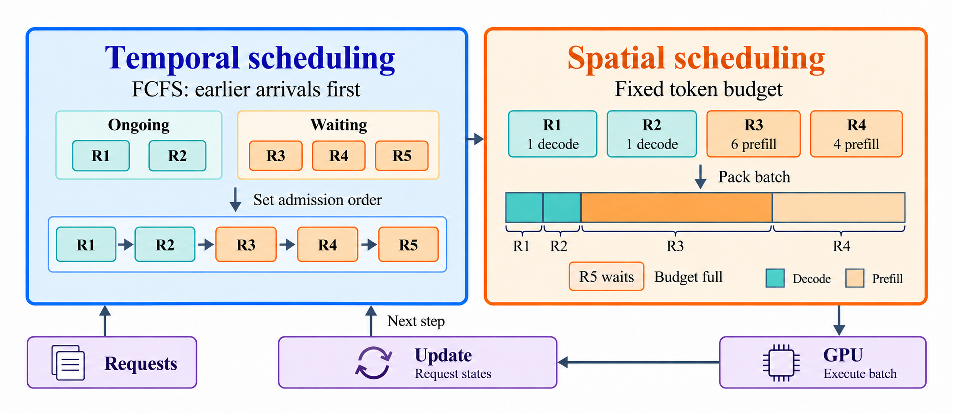
\includegraphics[width=\columnwidth]{figures/introduction/intro.pdf}
  \caption{Temporal and spatial scheduling in LLM serving.}
  \label{fig:serving-workflow}
\end{figure}


Existing throughput-oriented engines commonly use first-come-first-served (FCFS) admission for temporal scheduling and a fixed maximum token budget for spatial scheduling, without adapting these policies to the heterogeneous SLOs of individual requests.
To assess the impact of these policies, we evaluate vLLM's default FCFS scheduler on Qwen3-14B using the mathematical-reasoning workload with heterogeneous TTFT and TPOT requirements.
Among requests with tight TTFT SLOs, only 48.89\% satisfy both SLOs, with TTFT violations accounting for most failures.
For requests with tight TPOT SLOs, joint SLO attainment is similarly low at 12.00\%, with TPOT violations as the main cause.
Across the workload, only 53.48\% of requests satisfy both TTFT and TPOT SLOs.
This low joint attainment highlights the limitations of SLO-unaware scheduling under heterogeneous latency requirements.


First, SLO-unaware temporal scheduling leads to an admission order that does not reflect request urgency.
Under FCFS, a request with a tight TTFT objective can wait behind earlier requests with ample latency slack.
The urgent request may exhaust its TTFT budget in the queue, even though the earlier requests could tolerate being served later.
FCFS therefore misses the opportunity to defer less urgent requests and use their slack to reduce queueing delays for requests with tighter SLOs.


Second, existing spatial scheduling policies allocate tokens under a fixed per-step budget without considering the TPOT requirements of active decode requests.
Because decoding requests must wait for the entire batch to finish before receiving their next tokens, admitting more prefill work can prolong their inter-token delays.
With 2,048 decode tokens fixed, increasing prefill work from zero to 2,048 tokens raises mean step time from 329\,ms to 759\,ms.
Moreover, the same total token count can yield different step times: under a 4,096-token budget, pure-prefill and pure-decode steps take 611\,ms and 683\,ms, respectively, whereas an evenly mixed step takes 759\,ms.
A fixed token budget therefore cannot reliably bound step duration or adapt prefill allocation to the latency tolerance of decoding requests.

Addressing these inefficiencies requires coordinating request-level urgency with batch-level execution time.
First, temporal scheduling involves deciding which waiting requests to admit and which ongoing requests can be deferred under resource contention.
These requests are governed by different active SLOs and have consumed different portions of their latency budgets, so determining their execution order hinges on a consistent comparison of urgency across phases.
Second, spatial scheduling couples the latency requirements of prefill and decode requests through token allocation within a shared batch.
Allocating more tokens to prefill can advance requests with urgent TTFT objectives but also prolong the wait for decoding requests, whereas overly restricting prefill can leave those urgent requests waiting.
Balancing these competing demands requires accurately estimating step time under varying prefill/decode compositions and execution contexts, then using that estimate to guide per-step token allocation.


We therefore propose \tango{}, a multi-SLO LLM serving system that jointly controls temporal request dispatch and spatial token allocation.
\tango{} aims to improve goodput while satisfying heterogeneous TTFT and TPOT requirements.
It comprises a \dispatcher{} and a \allocator{}.
The \dispatcher{} assigns phase-aware deadlines according to each request's active SLO and uses them to guide admission and preemption, prioritizing requests with tighter latency budgets.
The \allocator{} uses a step-time model to predict the execution time of mixed prefill/decode batches and adjusts their prefill token budgets according to the remaining latency slack of decoding requests.


This paper makes three major contributions:
\begin{itemize}
  \item \textbf{Investigating scheduling inefficiencies in multi-SLO LLM serving.}
  The analysis motivates us to account for heterogeneous request urgency and mixed prefill/decode interference through joint control of request dispatch and token allocation.

  \item \textbf{The design of a \dispatcher{} that prioritizes requests across inference phases.}
  By mapping each request's active SLO to a comparable deadline, it guides request admission and preemption, mitigating temporal inefficiency caused by SLO-unaware queueing.

  \item \textbf{The design of a \allocator{} that adapts batch composition to latency constraints.}
  Based on predicted step time, it converts the remaining TPOT slack into a prefill token budget, mitigating mixed prefill/decode interference while preserving progress for requests with tight TTFT requirements.
\end{itemize}


We evaluate \tango{} against vLLM, SOLA, and JITServe using Llama-3.1-8B, Qwen3-14B, and Qwen3-32B under chatbot, mathematical-reasoning, and software-agent workloads.
Compared with state-of-the-art systems, \tango{} improves overall SLO attainment by 58.72\% and achieves $1.52\times$ the goodput on average.
